% Copyright 2004 by Till Tantau <tantau@users.sourceforge.net>.
%
% In principle, this file can be redistributed and/or modified under
% the terms of the GNU Public License, version 2.
%
% However, this file is supposed to be a template to be modified
% for your own needs. For this reason, if you use this file as a
% template and not specifically distribute it as part of a another
% package/program, I grant the extra permission to freely copy and
% modify this file as you see fit and even to delete this copyright
% notice. 

\documentclass{beamer}

% There are many different themes available for Beamer. A comprehensive
% list with examples is given here:
% http://deic.uab.es/~iblanes/beamer_gallery/index_by_theme.html
% You can uncomment the themes below if you would like to use a different
% one:
%\usetheme{AnnArbor}
%\usetheme{Antibes}
%\usetheme{Bergen}
%\usetheme{Berkeley}
%\usetheme{Berlin}
%\usetheme{Boadilla}
%\usetheme{boxes}
%\usetheme{CambridgeUS}
%\usetheme{Copenhagen}
%\usetheme{Darmstadt}
%\usetheme{default}
%\usetheme{Frankfurt}
%\usetheme{Goettingen}
%\usetheme{Hannover}
%\usetheme{Ilmenau}
%\usetheme{JuanLesPins}
%\usetheme{Luebeck}
\usetheme{Madrid}
%\usetheme{Malmoe}
%\usetheme{Marburg}
%\usetheme{Montpellier}
%\usetheme{PaloAlto}
%\usetheme{Pittsburgh}
%\usetheme{Rochester}
%\usetheme{Singapore}
%\usetheme{Szeged}
%\usetheme{Warsaw}

\title{¿Que ves cuando lo ves?}

% A subtitle is optional and this may be deleted
\subtitle{Optional Subtitle}

\author{Gonzalo Florio \and Ignacio Linari \and Cyntia Bonomi}
% - Give the names in the same order as the appear in the paper.
% - Use the \inst{?} command only if the authors have different
%   affiliation.

\institute[Universities of Somewhere and Elsewhere] % (optional, but mostly needed)
{
  \inst{1}%
  Departmento de Computación\\
  Universidad de Buenos Aires
  \and
  \inst{2}%
  Department of Theoretical Philosophy\\
  University of Elsewhere}
% - Use the \inst command only if there are several affiliations.
% - Keep it simple, no one is interested in your street address.

\date{Conference Name, 2013}
% - Either use conference name or its abbreviation.
% - Not really informative to the audience, more for people (including
%   yourself) who are reading the slides online

\subject{Theoretical Computer Science}
% This is only inserted into the PDF information catalog. Can be left
% out. 

% If you have a file called "university-logo-filename.xxx", where xxx
% is a graphic format that can be processed by latex or pdflatex,
% resp., then you can add a logo as follows:

% \pgfdeclareimage[height=0.5cm]{university-logo}{university-logo-filename}
% \logo{\pgfuseimage{university-logo}}

% Delete this, if you do not want the table of contents to pop up at
% the beginning of each subsection:
\AtBeginSubsection[]
{
  \begin{frame}<beamer>{Outline}
    \tableofcontents[currentsection,currentsubsection]
  \end{frame}
}

% Let's get started
\begin{document}

\begin{frame}
  \titlepage
\end{frame}

\begin{frame}{Outline}
  \tableofcontents
  % You might wish to add the option [pausesections]
\end{frame}

% Section and subsections will appear in the presentation overview
% and table of contents.
\section{First Main Section}

\subsection{Idea}

\begin{frame}{Hipotesis}{Optional Subtitle}
  \begin{itemize}
  \item {
  	
    %Nos preguntamos que identifican las personas cuando ven un logo? Colores? Conceptos? Formas? 

    Nos preguntamos que tan bien hacen su trabajo los logos de marcas. Las personas cuando los ven identifican Conceptos, Colores, formas, o no les significan nada especifico? 

  }

 
  \end{itemize}
\end{frame}

\subsection{Experimento}

% You can reveal the parts of a slide one at a time
% with the \pause command:
\begin{frame}{Experimento}
  \begin{itemize}
  \item {
    Conjunto de trials que muestran un logo target y luego 4 logos distintos relacionados con el targuet de acuerdo a 4 categorias: Forma/Letra, Concepto, Color, Ruido.   
    \pause % The slide will pause after showing the first item
  }
  \item {   
	Cada participante dado el logo targuet debe seleccionar segun su criterio de asociacion uno de los 4 logos. 
  }
  % or you can use the \uncover command to reveal general
  % content (not just \items):
%  \item<5-> {
%    Fifth item. \uncover<6->{Extra text in the fifth item.}
%  }
  \end{itemize}
\end{frame}

\section{Analisis de datos}

\subsection{Definiciones}

%Ir: Índice de relación en un trial = 
%# Ir_uxc: Índice de relación de un usuario respecto a una de las cuatro clases = Sum Ir %de los trials de ese usuario en los que eligió la clase c.

%# Ir_l1xl2: Índice de relación de un logo respecto a otro = Sum Ir de los trials con target l1 en los que se eligió a l2.


\begin{frame}{Metricas}
\begin{block}{Indice de Relacion en un trial}
IR = 1/tiempo.
\end{block}

\begin{block}{Indice de relacion de un usuario respecto a una clase.}
$IR\_uxc$ = $\sum IR$ de los trials de ese usuario en los que eligio la clase.
\end{block}

\begin{block}{Índice de relación de un choice(clase?) respecto a un target.}
$IR\_cxt$ = $\sum IR$ de los trials con el target t en los que se eligió el choice c.
\end{block}

\begin{block}{Índice de relación de un logo respecto a otro }
$IR\_l1xl2$ = $\sum IR$ de los trials con con target l1 en los que se eligió a l2.
\end{block}


%\begin{example}
%Here is an example of an example block.
%\end{example}
\end{frame}

\begin{frame}{Resultados}

\begin{figure}[h]
 \centering
  \begin{minipage}[c]{1\textwidth}
	\centering	
	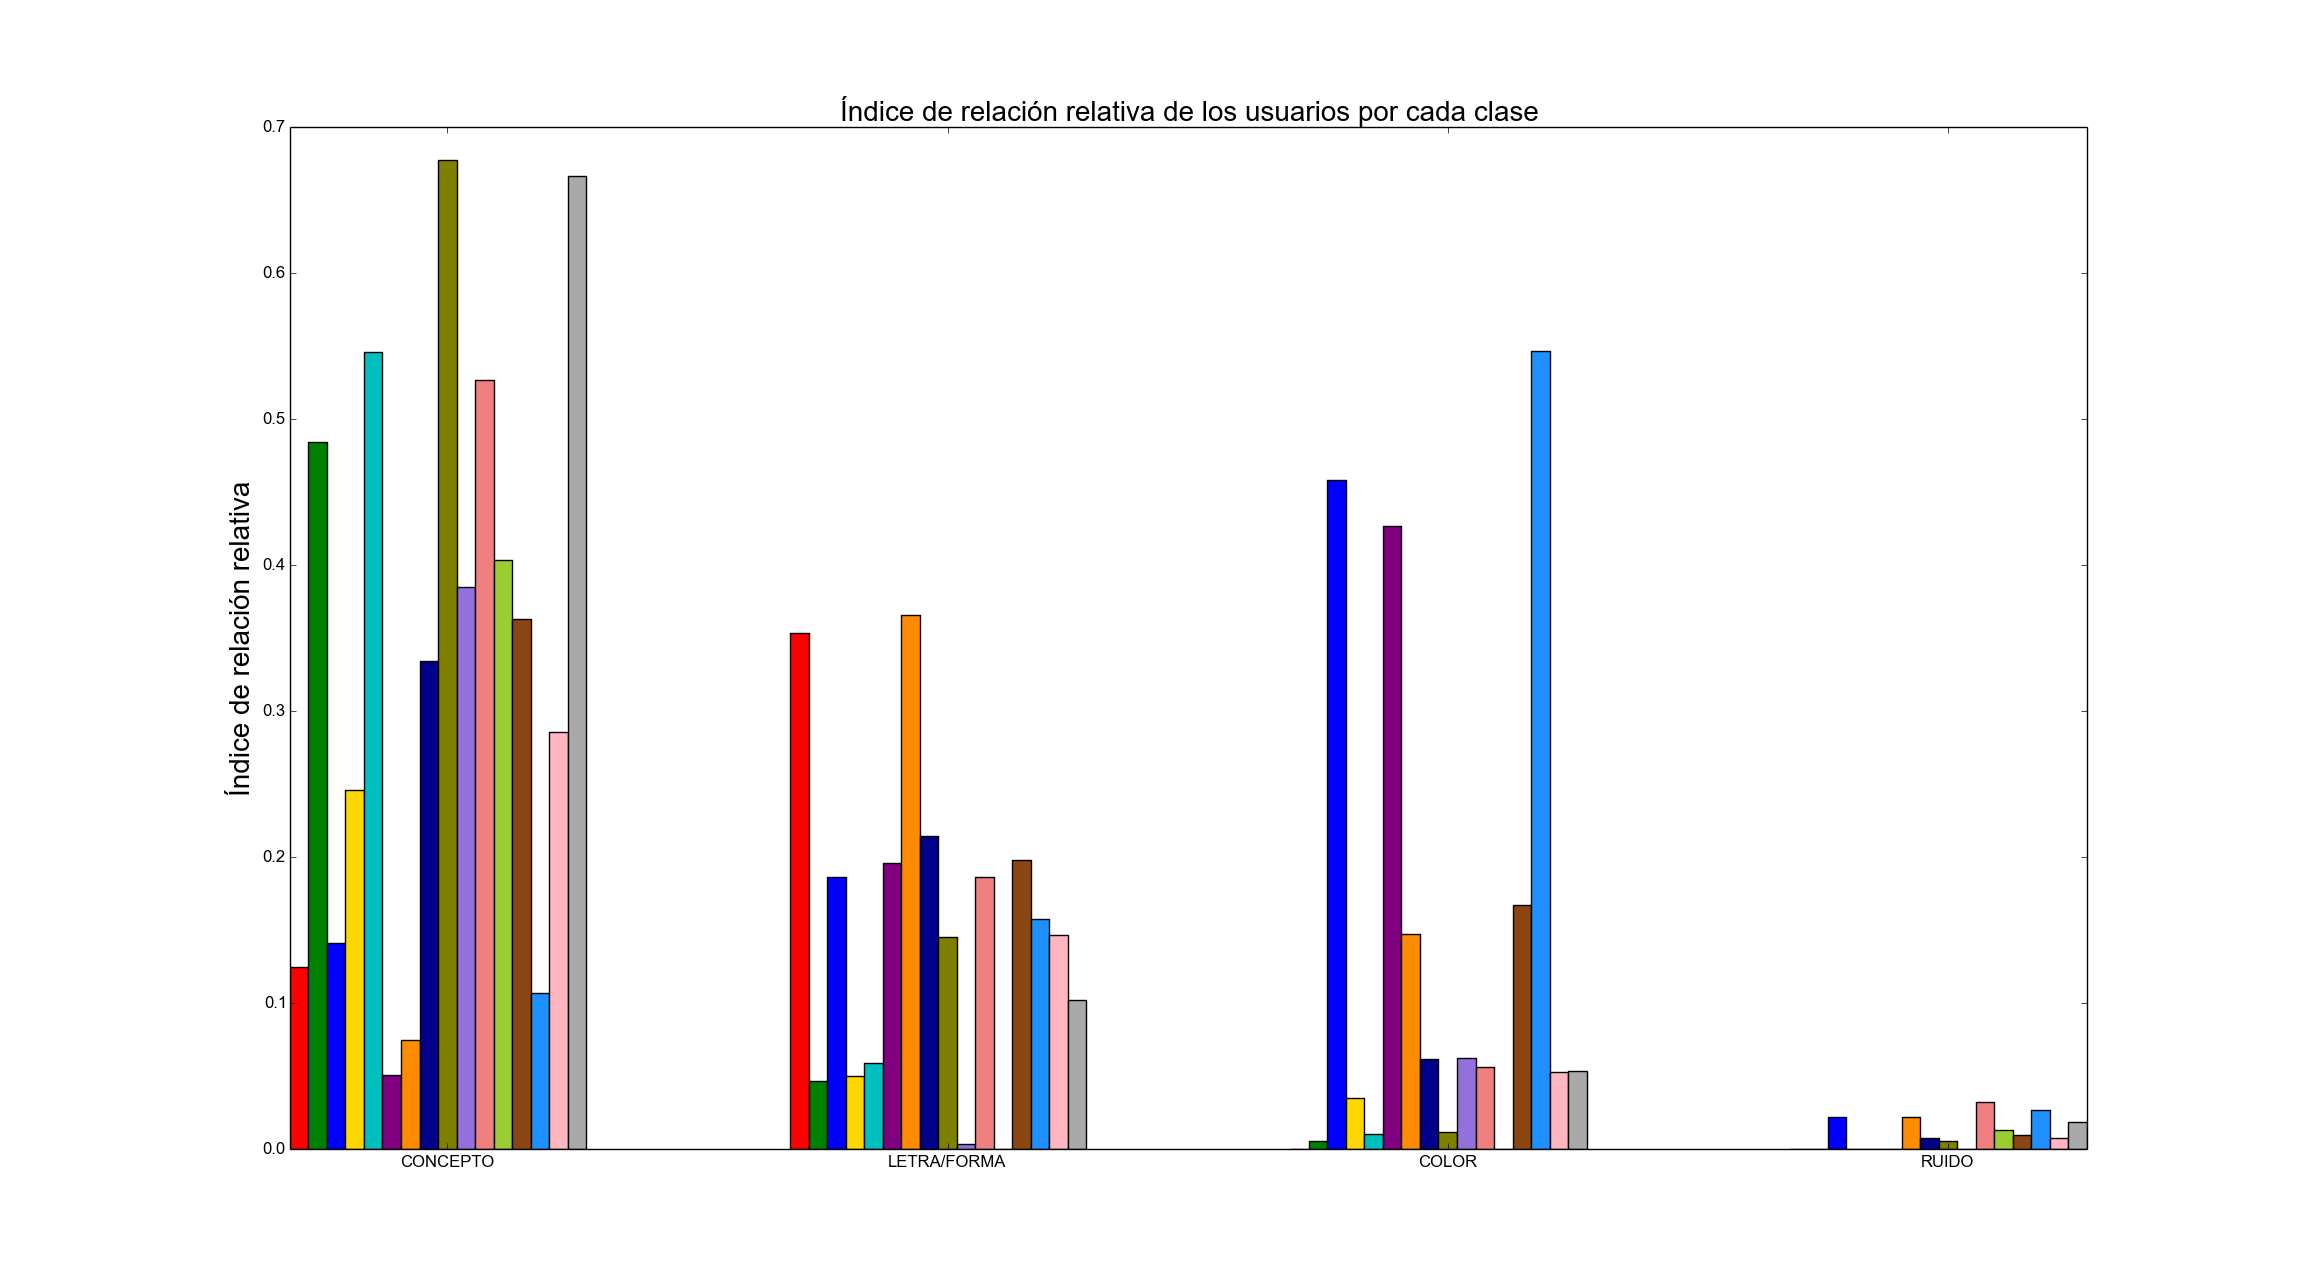
\includegraphics[scale=0.2]{irr_uxc.png}
        \caption{imagen}
  \end{minipage}
\end{figure}


\end{frame}

% Placing a * after \section means it will not show in the
% outline or table of contents.
\section*{Summary}

\begin{frame}{Summary}
  \begin{itemize}
  \item
    The \alert{first main message} of your talk in one or two lines.
  \item
    The \alert{second main message} of your talk in one or two lines.
  \item
    Perhaps a \alert{third message}, but not more than that.
  \end{itemize}
  
  \begin{itemize}
  \item
    Outlook
    \begin{itemize}
    \item
      Something you haven't solved.
    \item
      Something else you haven't solved.
    \end{itemize}
  \end{itemize}
\end{frame}



% All of the following is optional and typically not needed. 
\appendix
\section<presentation>*{\appendixname}
\subsection<presentation>*{For Further Reading}

\begin{frame}[allowframebreaks]
  \frametitle<presentation>{For Further Reading}
    
  \begin{thebibliography}{10}
    
  \beamertemplatebookbibitems
  % Start with overview books.

  \bibitem{Author1990}
    A.~Author.
    \newblock {\em Handbook of Everything}.
    \newblock Some Press, 1990.
 
    
  \beamertemplatearticlebibitems
  % Followed by interesting articles. Keep the list short. 

  \bibitem{Someone2000}
    S.~Someone.
    \newblock On this and that.
    \newblock {\em Journal of This and That}, 2(1):50--100,
    2000.
  \end{thebibliography}
\end{frame}

\end{document}


